\documentclass[twoside]{article}

\usepackage[preprint]{aistats2027}
\usepackage[round,authoryear]{natbib}
\usepackage{amsmath,amssymb,amsthm}
\usepackage{mathtools}
\usepackage{microtype}
\usepackage{booktabs}
\usepackage{tikz}
\usepackage{url}

\renewcommand{\bibname}{References}
\renewcommand{\bibsection}{\subsubsection*{\bibname}}
\bibliographystyle{apalike}

\newtheorem{theorem}{Theorem}
\newtheorem{lemma}[theorem]{Lemma}
\newtheorem{proposition}[theorem]{Proposition}
\newtheorem{corollary}[theorem]{Corollary}
\newcommand{\E}{\mathbb E}
\newcommand{\R}{\mathbb R}
\newcommand{\cH}{\mathcal H}
\newcommand{\FM}{\textnormal{\textsc{ForceMoM}}}
\newcommand{\one}{\mathbf 1}

\begin{document}
\runningtitle{Adaptation Frontier for Heavy-Tailed Bandits}

\twocolumn[
\aistatstitle{A Sharp Adaptation Frontier for Heavy-Tailed Bandits\\with Unknown Moments}

\aistatsauthor{Pahan Dewasurendra}

\aistatsaddress{Johns Hopkins University\\[4pt] July 28, 2026}
]

\begin{abstract}
Heavy-tailed bandit algorithms attain optimal regret when given a finite
moment order and its bound. Without either parameter, optimal adaptation is
impossible unless one restricts the reward distributions. What can be
achieved under the moment condition alone has remained open. We give a sharp
answer in the form of a Pareto frontier.

Our algorithm takes only an exploration exponent $\rho\in(0,1)$. It combines
deterministic forced exploration with a median-of-means empirical leader and
uses neither the moment order, its bound, nor a tail-sign condition. If the
unknown rewards have $(1+\epsilon)$th absolute moments bounded by $u$, its
worst-case regret is, up to explicit arm factors and an arbitrarily slow
factor,
\[
 u^{1/(1+\epsilon)}
 T^{1-\rho\epsilon/(1+\epsilon)},
\]
while its regret on every fixed instance is $O(T^\rho)$. A matching lower
bound shows that improving either polynomial exponent worsens the other.
Most notably, every fixed $\rho\leq2/3$ attains this frontier simultaneously
for all $\epsilon\in(0,1]$. Thus at any point on this common segment, unknown
tail order has no further polynomial price beyond unknown scale. This answers
the assumption-free rate question posed at COLT 2025 on the maximal common
segment and gives the first matching algorithm for the unknown-scale lower
tradeoff.
\end{abstract}

\section{Introduction}

Heavy-tailed multi-armed bandits model sequential decisions when rewards may
have infinite variance. In the standard formulation, every arm satisfies
\begin{equation}
 \E|X|^{1+\epsilon}\leq u,
 \qquad \epsilon\in(0,1],\quad u>0.
 \label{eq:moment-intro}
\end{equation}
When $\epsilon$ and $u$ are known, robust UCB and MOSS variants achieve the
optimal worst-case rate
$u^{1/(1+\epsilon)}T^{1/(1+\epsilon)}$, with the usual
$K^{\epsilon/(1+\epsilon)}$ factor
\citep{bubeck2013bandits}. \citet{wei2020minimax} sharpen the corresponding
minimax construction. Both parameters determine how much of an extreme
observation should be trusted.

In practice neither parameter is generally available. Recent work shows a
sharp qualitative obstruction. No algorithm can recover the known-parameter
rate uniformly over $u$, or uniformly over $\epsilon$, without further
distributional assumptions \citep{genalti2024adaptive}. Algorithms that do
recover it assume, for example, a favorable sign for every truncated tail of
an optimal arm, as in \citet{huang2022adaptive}, \citet{genalti2024adaptive},
and \citet{chen2025uniinf}. Another route assumes symmetry
\citep{tamas2024data}. Such conditions exclude simple one-sided heavy tails.

This leaves a basic question posed explicitly by
\citet{genalti2025open}: what are the best regret rates when both parameters
are unknown and no assumption beyond \eqref{eq:moment-intro} is imposed?
The question has two parts. One needs a lower bound that quantifies the cost
and an algorithm that attains it. A recent technical note gives an
unknown-$u$ tradeoff between worst-case and fixed-instance rates
\citep{genalti2025lower}, but no matching algorithm was known.

We close this gap. The answer is not one rate. It is a Pareto frontier
indexed by the desired fixed-instance exponent $\rho$. Write
$p=1+\epsilon$. Ignoring slowly varying factors, the frontier is
\begin{equation}
 \boxed{\begin{gathered}
 \text{fixed instance: }T^\rho,\\[-1mm]
 \text{worst case: }u^{1/p}T^{1-\rho(p-1)/p}
 \end{gathered}}
 \label{eq:frontier-intro}
\end{equation}
The two exponents satisfy the exact lower relation
\begin{equation}
 \rho+\frac{p}{p-1}\left(1-\rho\frac{p-1}{p}\right)
 =\frac{p}{p-1}.
 \label{eq:equality-intro}
\end{equation}

\paragraph{Algorithmic idea.}
The algorithm is deliberately simple. It reserves
$K^{1-\rho}t^\rho$ cyclic pulls for exploration by time $t$. On all other
rounds it chooses the largest median-of-means estimate computed only from
these dedicated samples. The number of median blocks grows arbitrarily
slowly. This construction avoids the central difficulty faced by adaptive
UCB methods. It never needs to turn an unknown moment condition into a
numerical confidence radius.

Two properties produce the frontier. On each exploitation round, the
expected gap of the empirical leader is at most its mean-estimation error,
which is
\[
 u^{1/p}\left(\frac{K^\rho L(t)}{t^\rho}\right)^{(p-1)/p}
\]
for an arbitrarily slow $L$. Summing gives the worst-case exponent in
\eqref{eq:frontier-intro}. On a fixed instance, the median block count tends
to infinity. The probability of choosing any suboptimal leader is then
summable, even though neither $p$ nor $u$ is known. Only forced pulls remain,
giving $T^\rho$ regret.

\paragraph{Contributions.}
\begin{itemize}
\item We give the first assumption-free algorithm with a uniform moment-free
finite-time regret bound when both heavy-tail parameters are unknown.
\item We prove worst-case and fixed-instance bounds for the same algorithm.
Together with the information-theoretic lower bound, they determine the
polynomial unknown-scale adaptation frontier.
\item One implementation with any $\rho\leq2/3$ is frontier-optimal for every
$p\in(1,2]$ simultaneously. This is the largest segment shared by all moment
orders and requires no knowledge of $p$.
\end{itemize}

\begin{table}[t]
\caption{Parameter adaptation under a finite $p$th absolute moment. ``Tail
sign'' denotes truncated non-negativity for losses or its reward analogue.
PF means parameter-free in both $p$ and $u$.}
\label{tab:comparison}
\centering
\scriptsize
\begin{tabular}{@{}llll@{}}
\toprule
Method & PF & Extra assumption & Guarantee\\
\midrule
Robust UCB & no & none & known-param. optimal\\
AdaTINF & yes & tail sign & worst-case optimal\\
AdaR-UCB & yes & tail sign & both near-optimal\\
uniINF & yes & tail sign & best of both worlds\\
RMM-UCB & yes & symmetry & both near-optimal\\
\FM{} & yes & none & sharp tradeoff\\
\bottomrule
\end{tabular}
\end{table}

\section{Setting and Adaptation Criteria}
\label{sec:setting}

There are $K\geq2$ arms. Pulls from arm $i$ are i.i.d. with law $\nu_i$
and mean $\mu_i$. At round $t$, a policy chooses $I_t$ from past actions and
observations, then observes an independent draw from $\nu_{I_t}$. Let
\[
 \mu_*=\max_i\mu_i,\qquad \Delta_i=\mu_*-\mu_i.
\]
The expected cumulative regret is
\[
 R_T(\nu)=\E_\nu\sum_{t=1}^T\Delta_{I_t}.
\]
For $p\in(1,2]$ and $u>0$, let
\[
 \cH_{p,u}=\{\nu: \E_{\nu_i}|X|^p\leq u\text{ for all }i\}.
\]
The policy is not given $p$, $u$, or an upper bound on either. Jensen's
inequality gives $|\mu_i|\leq u^{1/p}$ and $\Delta_i\leq2u^{1/p}$.

Following \citet{hadiji2023range} and \citet{genalti2025lower}, a
moment-free distribution-free bound $\Phi_p$ satisfies
\begin{equation}
 \sup_{\nu\in\cH_{p,u}}R_T(\nu)
 \leq u^{1/p}\Phi_p(T)
 \quad\text{for every }u,T.
 \label{eq:free-def}
\end{equation}
A distribution-dependent rate $\Psi$ satisfies
\begin{equation}
 \limsup_{T\to\infty}\frac{R_T(\nu)}{\Psi(T)}<\infty
 \quad\text{for every fixed }\nu.
 \label{eq:dep-def}
\end{equation}
Constants in \eqref{eq:dep-def} may depend on the instance. This distinction
is essential. Uniformly logarithmic instance-dependent regret is impossible
when the moment scale is unrestricted. This appears both in eventual
consistency results \citep{ashutosh2021letting} and in the sharp lower
tradeoff \citep{genalti2025lower}.

\section{A Parameter-Free Empirical Leader}
\label{sec:algorithm}

Fix $\rho\in(0,1)$. Let $\ell:\mathbb N\to[1,\infty)$ be nondecreasing,
$\ell(n)\to\infty$, $\ell(n+1)-\ell(n)\leq1$, and
$\log\ell(n)=o(\log n)$. The concrete choice
\begin{equation}
 \ell(n)=\log\log(e^e+n)
 \label{eq:ell}
\end{equation}
is sufficient. Define
\[
 m_0=\left\lceil16\log(2K+e)\right\rceil.
\]
The first $Km_0$ rounds pull every arm $m_0$ times. These and later forced
pulls form a dedicated exploration stream. Exploitation rewards are not used
for estimation.

After initialization, set the target total number of exploration pulls to
\begin{equation}
 D_t=\max\left\{Km_0,
 \left\lceil K^{1-\rho}t^\rho\right\rceil\right\}.
 \label{eq:target}
\end{equation}
At round $t$, force the next arm in cyclic order if fewer than $D_t$
exploration pulls have occurred. Otherwise exploit. The target rises by at
most one per round. Indeed, the derivative of
$K^{1-\rho}t^\rho$ is at most $\rho$ once $t\geq K$. Induction from the end
of initialization shows that the target is met exactly. Cyclic assignment
makes arm exploration counts differ by at most one. Consequently, each arm has at
least
\begin{equation}
 n_t=\left\lfloor D_{t-1}/K\right\rfloor
 \gtrsim (t/K)^\rho
 \label{eq:sample-growth}
\end{equation}
dedicated samples before an exploitation decision.

For $n\geq m_0$, let $q(n)$ be the largest odd integer no larger than
\begin{equation}
 \min\{n,\,2\lceil\log(2K)+\ell(n)\rceil+1\}.
 \label{eq:q}
\end{equation}
Split the first $q\lfloor n/q\rfloor$ samples into $q$ disjoint blocks,
average within each block, and take their median. Denote the resulting arm
estimate by $M_i(n)$. On an exploitation round, \FM{} chooses an arm with
largest $M_i(n_i)$.

The algorithm is anytime. It needs no numerical tail information. A direct
implementation is polynomial. Store arm-wise prefix sums and cache estimates
between exploration updates. Recomputing the $q(n)$ block means and their
median after a new dedicated sample costs $O(q(n))$ with linear-time median
selection. Through $n$ dedicated samples per arm, this is
$O(Kn\{\log K+\ell(n)\})$ work and $O(Kn)$ storage. Each leader scan costs
$O(K)$.

\subsection{A parameter-free MoM bound}

The same estimator works for every unknown $p$ because its tuning is only a
block count.

\begin{lemma}[Median-of-means envelope]
\label{lem:mom}
Let $X_1,\ldots,X_n$ be i.i.d. with mean $\mu$ and
$\E|X|^p\leq u$ for some $p\in(1,2]$. Form a median of $q\geq3$ odd block
means, where $q\leq n$, and write $k=(q+1)/2$. Then, for every $x>0$,
\begin{equation}
 \Pr\{|M_{n,q}-\mu|>x\}
 \leq \min\left\{1,
 \left(\frac{64u(q/n)^{p-1}}{x^p}\right)^k\right\}.
 \label{eq:mom-tail}
\end{equation}
Moreover,
\begin{equation}
 \E|M_{n,q}-\mu|
 \leq C u^{1/p}(q/n)^{(p-1)/p}
 \label{eq:mom-mean}
\end{equation}
for a universal constant $C$.
If $K$ arm estimates use block counts with
$k\geq\log(2K)$ and common upper bounds $q$ and $n^{-1}$, then
\begin{equation}
 \E\max_{i\leq K}|M_i-\mu_i|
 \leq C u^{1/p}(q/n)^{(p-1)/p}.
 \label{eq:mom-max}
\end{equation}
\end{lemma}

\begin{proof}
Jensen and convexity give
\[
 \E|X-\mu|^p
 \leq2^{p-1}\{\E|X|^p+|\mu|^p\}\leq2^pu.
\]
If a block has size $m=\lfloor n/q\rfloor$, the von Bahr--Esseen
inequality \citep{vonbahr1965inequalities} yields
\[
 \E|\bar X-\mu|^p
 \leq2^{p+1}um^{1-p}
 \leq16u(q/n)^{p-1}.
\]
The last step uses $m\geq n/(2q)$ and $p\leq2$. By Markov's inequality, one
block is bad at radius $x$ with probability at most
$16u(q/n)^{p-1}x^{-p}$. A bad median requires a set of $k$ bad blocks.
Independence of the disjoint blocks and a union bound over at most $2^q$
sets give \eqref{eq:mom-tail}, since $q=2k-1$ and $2^q\leq4^k$.

Let $x_0=64^{1/p}u^{1/p}(q/n)^{(p-1)/p}$. Integrating
\eqref{eq:mom-tail} gives
\[
 \E|M_{n,q}-\mu|
 \leq x_0+\int_{x_0}^\infty(x_0/x)^{pk}\,dx
 \leq2x_0,
\]
because $q\geq3$ implies $pk-1>1$. This proves
\eqref{eq:mom-mean}.

For $Z=\max_i|M_i-\mu_i|$, the union bound replaces the tail crossover
$x_0$ by at most $K^{1/(pk)}x_0$. Integrating again gives the same factor.
It is at most $e$ when $k\geq\log(2K)$. This proves
\eqref{eq:mom-max} without needing independence across arms.
\end{proof}

\section{Worst-Case Regret}
\label{sec:free}

The leader rule converts estimation error directly into regret. If $J_t$ is
the empirical leader and $i_*$ is optimal, then pointwise
\begin{align}
 \Delta_{J_t}
 &=\mu_*-\mu_{J_t}\nonumber\\
 &\leq |M_{i_*}-\mu_*|+|M_{J_t}-\mu_{J_t}|\nonumber\\
 &\leq2\max_i|M_i-\mu_i|.
 \label{eq:leader}
\end{align}
No confidence level is chosen by the algorithm.

\begin{theorem}[Finite-time parameter-free regret]
\label{thm:upper}
There is a universal constant $C$ such that \FM{}, for every
$\rho\in(0,1)$, $p\in(1,2]$, $u>0$, and $T\geq1$, satisfies, with
$\gamma_p=(p-1)/p$,
\begin{align}
 \sup_{\nu\in\cH_{p,u}}R_T(\nu)
 \leq C u^{1/p}\big\{&K\log(eK)
 \nonumber\\
 &+K^{1-\rho}T^\rho\nonumber\\
 &+K^{\rho\gamma_p}T^{1-\rho\gamma_p}
 L_T^{\gamma_p}\big\},
 \label{eq:upper}
\end{align}
where $L_T=1+\log(2K)+\ell(T)$. The policy is independent of $p$ and $u$.
\end{theorem}

\begin{proof}
There are at most $D_T$ exploration rounds after accounting for the initial
constant target. Since every gap is at most $2u^{1/p}$, their contribution
is bounded by
\begin{equation}
 R_T^E\leq C u^{1/p}\{K\log(eK)+K^{1-\rho}T^\rho\}.
 \label{eq:explore-main}
\end{equation}
On an exploitation round, all arm sample counts differ by at most one.
Equations \eqref{eq:q} and \eqref{eq:sample-growth} therefore permit the
common bounds
\[
 q_i\leq C L_t,
 \qquad n_i\geq cK^{-\rho}t^\rho.
\]
The initialization guarantees the block-count condition in
\eqref{eq:mom-max}. Combining that equation with \eqref{eq:leader} gives
\begin{equation}
 \E\Delta_{J_t}\leq
 C u^{1/p}K^{\rho(p-1)/p}
 L_t^{(p-1)/p}t^{-\rho(p-1)/p}.
 \label{eq:instant-main}
\end{equation}
Put $a=\rho(p-1)/p$. Since $a<1/2$, monotonicity of $L_t$ and integral
comparison imply
\[
 \sum_{t=1}^T L_t^{(p-1)/p}t^{-a}
 \leq2L_T^{(p-1)/p}T^{1-a}.
\]
Summing \eqref{eq:instant-main} and adding
\eqref{eq:explore-main} proves \eqref{eq:upper}. The same enlarged constant
covers horizons ending during initialization.
\end{proof}

For $\rho\leq2/3$, the exploitation exponent dominates the exploration
exponent for every $p\in(1,2]$ because
\[
 \rho\leq1-\rho(p-1)/p.
\]
Thus, up to $K$ and the arbitrarily slow $L_T$ factor, the
distribution-free exponent is
\begin{equation}
 a_p(\rho)=1-\rho\frac{p-1}{p}.
 \label{eq:free-exponent}
\end{equation}

\section{Fixed Instances and the Sharp Frontier}
\label{sec:frontier}

The slowly increasing block count, unnecessary for the expectation bound,
is what makes exploitation mistakes summable on every fixed instance.

\begin{theorem}[Fixed-instance regret]
\label{thm:instance}
For every fixed bandit instance with a finite $p$th absolute moment for some
$p>1$, \FM{} satisfies
\begin{equation}
 \sum_{t=1}^\infty
 \Pr\{t\text{ is exploit and }I_t\notin\arg\max_i\mu_i\}<\infty.
 \label{eq:summable}
\end{equation}
Consequently,
\begin{equation}
 \limsup_{T\to\infty}\frac{R_T(\nu)}{T^\rho}
 \leq K^{-\rho}\sum_{i=1}^K\Delta_i.
 \label{eq:instance}
\end{equation}
\end{theorem}

\begin{proof}
If a suboptimal arm $i$ with gap $\Delta_i$ is the empirical leader, either
its estimate overshoots by $\Delta_i/2$ or an optimal estimate undershoots
by that amount. Lemma~\ref{lem:mom} bounds each probability by
\begin{equation}
 2\left[
 \frac{C u \overline q_t^{p-1}}
 {\Delta_i^p n_t^{p-1}}
 \right]^{(\underline q_t+1)/2}.
 \label{eq:fixed-tail}
\end{equation}
Here $n_t\gtrsim t^\rho$, the smaller block count
$\underline q_t\to\infty$, and the larger count satisfies
$\overline q_t\leq\underline q_t+2$ and
$\log\overline q_t=o(\log n_t)$. For fixed $p,u,\Delta_i$, the logarithm of
the bracket in \eqref{eq:fixed-tail} is eventually at most
$-(p-1)\log n_t/2$. Since $n_t\gtrsim t^\rho$, it is then at most
$-(p-1)\rho\log t/4$. Finally, $\underline q_t\to\infty$, so the complete
right side is at most $2t^{-3}$ for all sufficiently large $t$. Summing over
time and over the finitely many suboptimal arms proves \eqref{eq:summable}.

It remains to count forced pulls. Cyclic assignment gives each arm
$K^{-1}D_T+O(1)$ such pulls. Since
$D_T=K^{1-\rho}T^\rho+o(T^\rho)$, their regret divided by $T^\rho$ converges
to $K^{-\rho}\sum_i\Delta_i$. The exploitation regret is bounded because
\eqref{eq:summable} holds and all gaps are fixed. This proves
\eqref{eq:instance}.
\end{proof}

We now compare the two upper bounds with the information-theoretic
constraint. The following form is due to \citet{genalti2025lower}, adapting
the range argument of \citet{hadiji2023range}. We include a proof in the
supplement because it is central to the conclusion.

\begin{theorem}[Unknown-scale lower tradeoff]
\label{thm:lower}
Fix $p\in(1,2]$. Suppose a policy, without knowing $u$, has a moment-free
distribution-free bound $\Phi_p(T)=o(T)$ as in \eqref{eq:free-def}. Then on
every fixed instance $\nu$ with at least one suboptimal arm,
\begin{equation}
 \liminf_{T\to\infty}
 \frac{R_T(\nu)}{(T/\Phi_p(T))^{p/(p-1)}}
 \geq c_p\sum_{i:\Delta_i>0}\Delta_i,
 \label{eq:lower-tradeoff}
\end{equation}
where $c_p>0$ depends only on $p$.
Hence polynomial exponents $a$ and $b$ in
$\Phi_p(T)=T^{a+o(1)}$ and $\Psi(T)=T^{b+o(1)}$ must satisfy
\begin{equation}
 b+\frac{p}{p-1}a\geq\frac{p}{p-1}.
 \label{eq:exponent-lower}
\end{equation}
\end{theorem}

\begin{proof}
Fix a suboptimal arm $i$ with gap $\Delta_i$. For $\beta\in(0,1/2)$, replace
its law by
\begin{equation}
 \nu'_{i,\beta}=(1-\beta)\nu_i+
 \beta\delta_{\mu_i+2\Delta_i/\beta}.
 \label{eq:lower-alternative-main}
\end{equation}
Its new mean is $\mu_*+\Delta_i$. Let $v$ be a finite common $p$th-moment
bound for the original instance and take
$v'_\beta=v+(1-\beta)\E_{\nu_i}|X|^p+
\beta|\mu_i+2\Delta_i/\beta|^p$. This bounds every arm of the alternative and
satisfies
\begin{equation}
 (v'_\beta)^{1/p}
 =2\Delta_i\beta^{-(p-1)/p}\{1+o(1)\}
 \quad(\beta\downarrow0).
 \label{eq:lower-moment-main}
\end{equation}
Moreover,
$\mathrm{KL}(\nu_i,\nu'_{i,\beta})\leq\log(1/(1-\beta))
\leq2\beta\log2$.

Let $P,P'$ denote the two history laws and let $N_i(T)$ count pulls of arm
$i$. Data processing applied to the action at an independent uniform round,
followed by
$\operatorname{kl}(x,y)\geq(1-x)\log(1/(1-y))-\log2$, gives
\begin{align}
 &\left(1-\frac{v^{1/p}\Phi_p(T)}{T\Delta_i}\right)
 \log\frac{T\Delta_i}{(v'_\beta)^{1/p}\Phi_p(T)}-\log2
 \nonumber\\
 &\hspace{27mm}\leq2\beta\log2\,\E_PN_i(T).
 \label{eq:lower-key-main}
\end{align}
Here the regret guarantee bounds $\E_PN_i(T)$ on the original instance and
$T-\E_{P'}N_i(T)$ on the alternative.

Put $r=p/(p-1)$, $\alpha=8^{-r}$, and
$\beta_T=\alpha^{-1}(\Phi_p(T)/T)^r$. By \eqref{eq:lower-moment-main}, the
denominator inside the logarithm in \eqref{eq:lower-key-main} is
$\Delta_iT\{1+o(1)\}/4$. Its left side therefore tends to $\log2$, while
$\beta_T\to0$. It follows that
\[
 \liminf_{T\to\infty}
 \frac{\E_PN_i(T)}{(T/\Phi_p(T))^r}
 \geq\frac1{2\,8^r}.
\]
Multiplying by $\Delta_i$ and summing over suboptimal arms proves
\eqref{eq:lower-tradeoff}. The exponent relation follows by taking powers of
$T$.
\end{proof}

Substituting \eqref{eq:free-exponent} into
\eqref{eq:exponent-lower} forces $b\geq\rho$. Theorem~\ref{thm:instance}
attains $b=\rho$. We have therefore proved the main result.

\begin{corollary}[Simultaneous sharp frontier]
\label{cor:frontier}
Fix any $\rho\in(0,2/3]$. One policy, independent of $p$ and $u$, attains
for every $p\in(1,2]$ the polynomial exponents
\[
 (a_p,b)=\left(1-\rho\frac{p-1}{p},\rho\right).
\]
These exponents satisfy the lower tradeoff with equality for every $p$.
The slowly varying gap in \eqref{eq:upper} can be made arbitrarily small by
the choice of $\ell$.
\end{corollary}

\begin{figure}[t]
\centering
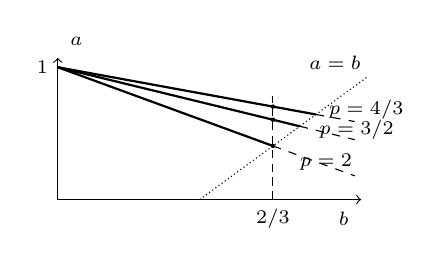
\begin{tikzpicture}[x=4.1cm,y=3.0cm]
 \draw[->] (0,0.44) -- (0.94,0.44)
   node[below left=1pt,font=\scriptsize] {$b$};
 \draw[->] (0,0.44) -- (0,1.04)
   node[above right=1pt,font=\scriptsize] {$a$};
 \draw[densely dotted] (0.44,0.44) -- (0.96,0.96)
   node[above left=-1pt,font=\scriptsize] {$a=b$};
 \draw[thick] (0,1) -- (0.6667,0.6667);
 \draw[dashed] (0.6667,0.6667) -- (0.92,0.54);
 \draw[thick] (0,1) -- (0.75,0.75);
 \draw[dashed] (0.75,0.75) -- (0.92,0.6933);
 \draw[thick] (0,1) -- (0.8,0.8);
 \draw[dashed] (0.8,0.8) -- (0.92,0.77);
 \draw[densely dashed] (0.6667,0.44) -- (0.6667,0.88);
 \fill (0.6667,0.6667) circle (0.8pt);
 \fill (0.6667,0.7778) circle (0.8pt);
 \fill (0.6667,0.8333) circle (0.8pt);
 \node[font=\scriptsize,anchor=west] at (0.81,0.82) {$p=4/3$};
 \node[font=\scriptsize,anchor=west] at (0.78,0.735) {$p=3/2$};
 \node[font=\scriptsize,anchor=west] at (0.72,0.60) {$p=2$};
 \node[font=\scriptsize,below] at (0.6667,0.44) {$2/3$};
 \node[font=\scriptsize,left] at (0,1) {$1$};
\end{tikzpicture}
\caption{Exponent geometry. The lower bound requires
$a\geq1-b(p-1)/p$. Thick segments are matched by \FM{} until each line meets
$a=b$. The vertical line at $b=2/3$ marks the endpoint of the largest segment
shared by every $p\in(1,2]$. Its dots show the three orders displayed.}
\label{fig:frontier}
\end{figure}

The same result also closes the entire relevant unknown-scale tradeoff when
the order may be used only to choose the design point.

\begin{corollary}[Order-aware unknown-scale frontier]
\label{cor:scale-frontier}
Fix $p\in(1,2]$ and $\rho\leq p/(2p-1)$. Then \FM{} with design exponent
$\rho$ uses no scale information and attains
\[
 (a_p,b)=\left(1-\rho\frac{p-1}{p},\rho\right),
\]
which meets \eqref{eq:exponent-lower} with equality. The balanced choice
$\rho_p^*=p/(2p-1)$ gives, up to $L_T$,
\begin{equation}
 R_T\leq C u^{1/p}
 K^{(p-1)/(2p-1)}T^{p/(2p-1)}L_T^{(p-1)/p}
 \label{eq:balanced-scale}
\end{equation}
apart from the additive initialization term, and has the same fixed-instance
polynomial exponent.
\end{corollary}

\begin{proof}
The restriction on $\rho$ is exactly
$\rho\leq1-\rho(p-1)/p$, so the exploitation term in
Theorem~\ref{thm:upper} dominates. Substitution in
Theorem~\ref{thm:lower} proves sharpness. At $\rho=p/(2p-1)$, the exploration
and exploitation powers of both $K$ and $T$ agree, giving
\eqref{eq:balanced-scale}.
\end{proof}

\begin{table}[t]
\caption{Polynomial exponent pairs $(a,b)$ for worst-case and fixed-instance
regret. Logarithmic fixed-instance regret is recorded as $b=0$. The last
column uses one policy with $\rho=2/3$ for every unknown $p$.}
\label{tab:exponents}
\centering
\scriptsize
\begin{tabular}{@{}cccc@{}}
\toprule
$p$ & known $p,u$ & unknown $u$, $p$-aware & both unknown\\
\midrule
$2$ & $(1/2,0)$ & $(2/3,2/3)$ & $(2/3,2/3)$\\
$3/2$ & $(2/3,0)$ & $(3/4,3/4)$ & $(7/9,2/3)$\\
$4/3$ & $(3/4,0)$ & $(4/5,4/5)$ & $(5/6,2/3)$\\
$p\downarrow1$ & $(1,0)$ & $(1,1)$ & $(1,2/3)$\\
\bottomrule
\end{tabular}
\end{table}

If $p$ were known but $u$ were not, balancing the two exponents would use
$\rho=p/(2p-1)$ and produce $T^{p/(2p-1)}$. No single fixed $\rho$ of this
form works for all $p$. Corollary~\ref{cor:frontier} instead identifies the
entire common frontier. Its largest point is $\rho=2/3$, where
\[
 a_p(2/3)=1-\frac{2(p-1)}{3p}.
\]
For finite variance this gives the sharp balanced $T^{2/3}$ rate. For
heavier tails the worst-case rate approaches linear smoothly.

Table~\ref{tab:exponents} separates two claims that can otherwise be confused.
Knowing $p$ permits selecting a different balanced point for each order.
Without $p$, the choice $\rho=2/3$ instead fixes the same instance exponent
for all orders and is sharp at that point for every $p$. The latter does not
claim to reproduce the $p$-aware balanced point when $p<2$.

There is no contradiction with the separate lower bound for adaptation to
$p$ at fixed $u$ \citep{genalti2024adaptive}. That benchmark is the faster
known-scale rate $T^{1/p}$. Here the unknown scale has already enlarged the
frontier. The same algorithm shows that learning $p$ requires no additional
polynomial loss along its common portion.

\section{Related Work and Discussion}
\label{sec:related}

\paragraph{Known parameters.}
\citet{bubeck2013bandits} introduced robust UCB based on truncation,
median-of-means, and Catoni estimators. Later algorithms sharpened the
worst-case logarithmic factors \citep{wei2020minimax}. Randomized policies
were developed by \citet{agrawal2021regret} and \citet{park2026boltzmann}.
These methods tune their estimators or indices using the moment parameters.
In particular, H-BE requires both $p$ and $u$ despite its closed-form action
probabilities \citep{park2026boltzmann}.
Recent adversarial best-of-both-worlds methods can remove the tail-sign
condition, but their clipping and learning rates explicitly use the moment
order and scale \citep{zhao2025linear}.

\paragraph{Parameter-free methods with assumptions.}
AdaTINF and AdaR-UCB adapt to both parameters under truncated tail-sign
conditions in \citet{huang2022adaptive} and \citet{genalti2024adaptive}.
uniINF obtains a best-of-both-worlds guarantee under the same condition
\citep{chen2025uniinf}. RMM-UCB instead assumes symmetry
\citep{tamas2024data}. These results seek the known-parameter optimum. Our
goal is different. We impose no shape or sign condition and characterize
the unavoidable loss.

\paragraph{Unrestricted adaptation.}
R-UCB-MoM is parameter-oblivious and eventually consistent over a broad
class, but its guarantee starts after an instance-dependent threshold and
does not provide a finite-time moment-free worst-case rate
\citep{ashutosh2021letting}. The forced-exploration architecture itself has
been studied for sub-Gaussian rewards \citep{han2024forced}. Replacing the
empirical mean is not enough for our result. The diverging MoM block count
and dedicated exploration stream are what yield both a uniform finite-time
bound and summable fixed-instance errors under every unknown $p>1$.

\paragraph{Scope.}
The frontier is polynomial. Arbitrarily slow factors remain between the
upper bound and \eqref{eq:lower-tradeoff}. Removing them while retaining one
algorithm for all $p$ is open. It is also open whether one parameter-free
policy can adapt among the order-specific frontier points beyond the common
range $\rho\leq2/3$. Our result concerns stochastic finite-armed bandits.
Adversarial, contextual, and linear variants require different tools.

\section{Conclusion}

Unknown heavy-tail parameters do not make regret minimization hopeless, but
they change its objective. There is an exact tradeoff between protection
against an unrestricted moment scale and fast learning on fixed instances.
A forced-exploration median leader attains that tradeoff without estimating
either tail parameter. The same policy is exponent-optimal for every finite
moment order, resolving the assumption-free adaptation question on the
common Pareto frontier.

\bibliography{references}

\section*{Checklist}
\begin{enumerate}
\item For all models and algorithms presented, check if you include:
\begin{enumerate}
\item A clear description of the mathematical setting, assumptions, algorithm, and/or model. [Yes/No/Not Applicable]

\textbf{Yes.} Sections 2 and 3 define the bandit classes, regret criteria, exploration schedule, estimator, and policy.

\item An analysis of the properties and complexity (time, space, sample size) of any algorithm. [Yes/No/Not Applicable]

\textbf{Yes.} Theorems 2 and 3 give finite-time and fixed-instance regret. Section 3 discusses an efficient implementation.

\item (Optional) Anonymized source code, with specification of all dependencies, including external libraries. [Yes/No/Not Applicable]

\textbf{Not Applicable.} No computational claim depends on code.
\end{enumerate}

\item For any theoretical claim, check if you include:
\begin{enumerate}
\item Statements of the full set of assumptions of all theoretical results. [Yes/No/Not Applicable]

\textbf{Yes.} Every theorem states its moment, horizon, arm, and algorithm conditions.

\item Complete proofs of all theoretical results. [Yes/No/Not Applicable]

\textbf{Yes.} The main text gives proof arguments and the supplement gives complete proofs, including the lower bound.

\item Clear explanations of any assumptions. [Yes/No/Not Applicable]

\textbf{Yes.} Sections 1, 2, and 7 contrast the sole moment condition with tail-sign and symmetry assumptions.
\end{enumerate}

\item For all figures and tables that present empirical results, check if you include:
\begin{enumerate}
\item The code, data, and instructions needed to reproduce the main experimental results. [Yes/No/Not Applicable]

\textbf{Not Applicable.} The paper contains no empirical results.

\item All the training details. [Yes/No/Not Applicable]

\textbf{Not Applicable.}

\item A clear definition of statistics and error bars. [Yes/No/Not Applicable]

\textbf{Not Applicable.}

\item A description of the computing infrastructure used. [Yes/No/Not Applicable]

\textbf{Not Applicable.}
\end{enumerate}

\item If you are using existing assets or curating/releasing new assets, check if you include:
\begin{enumerate}
\item Citations of the creator if your work uses existing assets. [Yes/No/Not Applicable]

\textbf{Not Applicable.}

\item The license information of the assets, if applicable. [Yes/No/Not Applicable]

\textbf{Not Applicable.}

\item New assets either in the supplemental material or as a URL, if applicable. [Yes/No/Not Applicable]

\textbf{Not Applicable.}

\item Information about consent from data providers/curators. [Yes/No/Not Applicable]

\textbf{Not Applicable.}

\item Discussion of sensible content if applicable. [Yes/No/Not Applicable]

\textbf{Not Applicable.}
\end{enumerate}

\item If you used crowdsourcing or conducted research with human subjects, check if you include:
\begin{enumerate}
\item The full text of instructions given to participants and screenshots. [Yes/No/Not Applicable]

\textbf{Not Applicable.}

\item Descriptions of potential participant risks and IRB approvals if applicable. [Yes/No/Not Applicable]

\textbf{Not Applicable.}

\item The estimated hourly wage paid to participants and total compensation. [Yes/No/Not Applicable]

\textbf{Not Applicable.}
\end{enumerate}
\end{enumerate}

\end{document}
